\chapter{Model Validation and Simulation}
\label{ch:model}

The model attempts to recreate a microgrid which uses some form of DER as a primary power source along side energy storage in order power the load. \autoref{fig:abridged_flow_diagram} shows a simplified flow diagram of the model using an ORC for the DER. The components include a ORC as a source, a load, a form of energy storage, and an inverter to link the energy storage with other pieces. In the figure, the blue blocks and lines represent electrical components, while green represents the flow of data. The ORC block is made up of heat exchangers, an isentropic pump, an isentropic expander, and an induction generator. 
The load block \verb|one line description of load|. 
The energy storage block \verb|one line description of energy storage|. 
The inverter block \verb|one line description of inverter|.

\begin{figure}[h]
	\centering
	\caption{A simplified diagram of power and data flows of the model. Blue lines represent electrical power connections and flows similar to a one-line diagram. Green boxes represent data flow from one part of the model to another.}
	\label{fig:abridged_flow_diagram_label}
	
	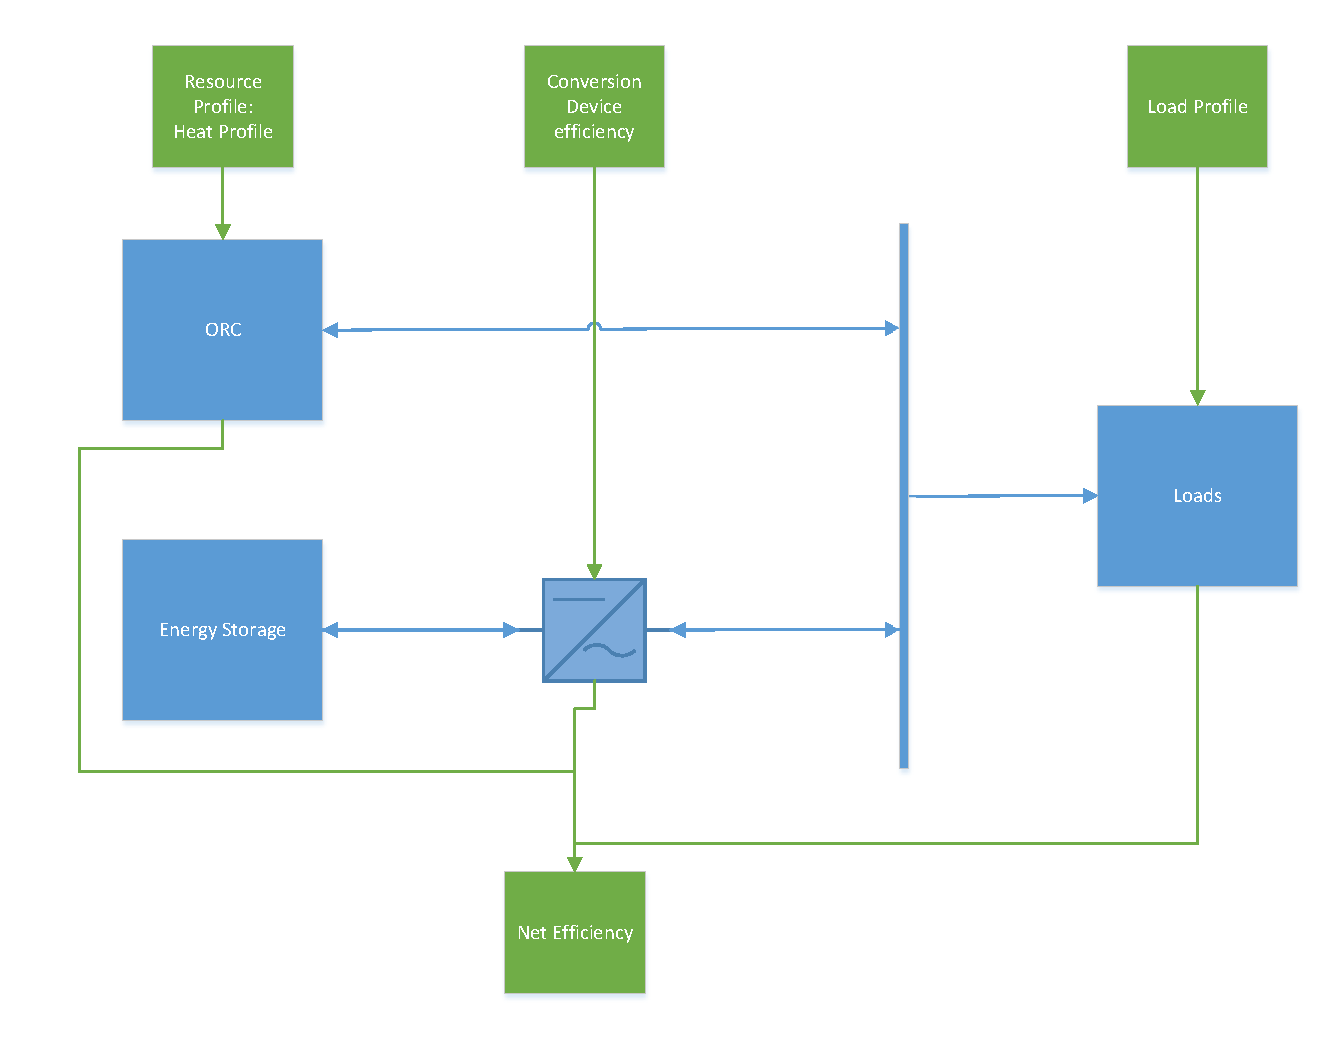
\includegraphics[width=\textwidth]{figures/Abridged Pilgrim Model Flow diagram - AC bus.pdf} 
	%\includegraphics[width=\textwidth]{figures/SimpleFlowDiagram.pdf}

\end{figure}

\section{Organic Rankine Cycle Generator}
The ORC generator block links the thermal, mechanical, and electric components of them model. The thermal properties of the fluids were obtained from a Matlab wrapper of the CoolProp library. \cite{Bell2014}

\subsection{Evaporator and Condenser}
The evaporator and the condenser are both represented using a heat exchanger script.  The function takes as inputs parameters about the high and low temperature fluids, specifically the inlet temperatures or enthalpies ($\si{\kelvin}$ or $\si{\joule\per\kilogram}$), mass flow rates ($\si{\kilogram\per\second} $), inlet pressures ($\si{\pascal}$), and fluid names, as well as parameters about the exchanger itself such as the overall heat transfer coefficient ($\si{\watt\per\kelvin\per\meter\squared}$), the heat transfer area ($\si{\meter\squared}$), and the heat exchanger type (e.g. counter or parallel flow). The function output is made up of the heat flow rate ($\si{\watt}$), and the temperatures or enthalpies at the outlets ($\si{\kelvin}$ or $\si{\joule\per\kilogram}$). 

In order to calculate the desired values, the Number of Transfer Units (NTU) method is used. Described in The Fundamentals of Heat and Mass Transfer, \cite{Incropera} this process calculates the output heat flow, $\dot{Q}$, relative to a theoretical maximum heat flow, $\dot{Q}_{max}$. This potential heat flow would be realized using an infinitely long counter flow geometry and is calculated as
\begin{equation}
\dot{Q}_{max} = C_{min}\left(T_{h,i} - T_{c,i}\right)
\end{equation}
where $C_{min}$ is the smaller heat capacity rate of the hot and cool fluids and $T_{h,i}$ and $T_{c,i}$ are the inlet temperatures of hot and cool fluids respectively. The heat capacity rate is the product of mass flow rate, $ \dot{m} $, and the mass specific heat at constant pressure, $ c_p $. 

The heat flow rates of the hot and cool fluids are related by the effectiveness, $\epsilon$, which is defined as 
\begin{equation}
\label{eq:effectiveness_def}
\epsilon \equiv \frac{\dot{Q}}{\dot{Q}_{max}}
\end{equation}

Numerically, the value of $\epsilon$ is a function of the ratio of the fluids' heat capacities, $C_r = \frac{C_{min}}{C_{max}}$, as well as the exchanger's Number of Transfer Units, $NTU = \frac{U \cdot A}{C_{min}}$, where $U$ is the overall heat transfer coefficient and $A$ is the total heat transfer area. Additionally, the direction of fluid flow changes the method of calculation. In parallel flow heat exchangers, the effectiveness is calculated as
\begin{equation}
\epsilon = \frac{1 - \exp\left[-NTU\left(1 + C_r\right)\right]}{1 + C_r}
\end{equation}
while counter flow devices use
\begin{equation}
\epsilon = \frac{1 - \exp\left[-NTU\left(1 - C_r\right)\right]}{1 - C_r\exp\left[-NTU\left(1 - C_r\right)\right]}
\end{equation}

Once the effectiveness and maximum heat transfer rate are determined, equation \ref{eq:effectiveness_def} is used to calculate the actual rate of heat flow, $\dot{Q}$. Finally, the change in temperature for each fluid is calculated based on their respective heat capacity rates at initial conditions and the rate of heat flowing between them. 
If the change in temperature for either fluid would result in vaporization or condensation, then the values must be recalculated because the specific heat is effectively infinite while the fluid is changing states. 

First, the heat flow rate necessary to have the fluid begin changing its state is determined and the fraction of this value relative to initial heat flow rate is calculated. 
The heat transfer area is reduced by this fraction and the function is re-run inputing the state of the two fluids as the one fluid begins to change phase. If enough heat flows between the two fluids such that the one completes the phase change, then the function is run a third time with the heat transfer area modified again. 

Within this script there are certain assumptions made in order to calculate the output values. The function will not return accurate results if both fluids simultaneously undergo a phase change because the ratio of heat capacities, $C_r$, will be undefined. Additionally, Ambient temperature and associated heat flow to the external environment is not accounted for in the script. Finally, it is assumed the pressure drop from inlet to outlet is negligible for both the high and low temperature fluids. 

\subsubsection{Expander and Pump}
The expander/turbine and pump components are both modeled by a fluid undergoing non-ideal isentropic expansion or compression. For an ideal isentropic process, the fluid will experience some thermodynamic changes while its internal entropy remains constant. 

The function takes as inputs certain properties of the fluid, such as the inlet temperature or enthalpy ($\si{\kelvin}$ or $\si{\joule\per\kilogram}$), both the inlet and outlet pressures ($\si{\pascal}$), and the mass flow rate ($\si{\kilogram\per\second}$). Also needed is the isentropic efficiency, a unitless parameter of the machine which describes lost power due to deviations from the ideal insentropic process. The function returns the power produced or consumed\footnote{Power is produced if the pressure at the inlet is greater than at the outlet, and consumed if inlet pressure is less than that of the outlet.} ($\si{\watt}$) and the temperature or enthalpy ($\si{\kelvin}$ or $\si{\joule\per\kilogram}$) of the fluid at the outlet.

Using the inputs and the Cool Prop library, the Mass Specific Entropy, $S$, of the fluid is determined for the fluid at the inlet. In an ideal process, this value would remain constant, so it is used to determine the ideal enthalpy of the outlet. Next the ideal power transferred is calculated as 
\begin{equation}
\label{eq:power_enthalpy}
P = \dot{m} \left(H_i - H_o\right)
\end{equation}
where $H_i$ and $H_o$ are the inlet and outlet enthalpies respectively.

To obtain the actual transfered power, the isentropic efficiency is applied to the ideal power such that the ideal is necessarily greater than the actual. When the value of $H_i$ is larger than $H_o$, $P$ is positive\footnote{Power is produced.} therefore efficiency is multiplied. When $H_i$ is less than $H_o$, $P$ is negative\footnote{Power is consumed.} and ideal power is divided by efficiency. After actual transferred power is calculated, equation \ref{eq:power_enthalpy} is used to find $H_o$ and the fluid temperature at the outlet.

\subsection{Induction Generator}
The generator block models a Squirrel Cage Induction Generator (SCIG) in order to convert the mechanical power to an electrical form. Depending on the microgrid design, this could also be achieved by modeling other types of generators such as a DC generator, synchronous generator, or an alternate form of induction generator. 

This function block takes several electrical and mechanical parameters as inputs such as the line to line voltage ($\si{\volt}$) and electrical frequency ($\si{\hertz}$) at the leads, the mechanical speed at the shaft ($\si{\rpm}$), and the number pole pairs in machine's windings. Also input are the resistive and inductive impedances ($\si{\ohm}$) of the stator, rotor, and core, as well as the capacitive impedance and equivalent series resistance of external excitation capacitor. The function returns the active ($\si{\watt}$) and reactive ($\si{\voltampreactive}$) power outputs and losses.

\begin{figure}[h]
	
\centering

\begin{tikzpicture}[american voltages]
\draw[color=black, thick]
%Input
(0,0) to [open, l=$V_{ph}$, o-o] (0,4){}

%low
(0,0) -- (9,0){}

%stator
(0,4) -- (1.5,4) to [R, l=$R_{s}$] (3,4) to [L, l = $j X_{s}$] (4.5,4){}

%rotor
(4.5,4) -- (5.5,4) to [R, l=$R_{r}$] (7.5,4) to [L, l = $j X_{r}$] (9,4) to [R, l=$R_{r}\frac{1-s}{s}$] (9,0){}

%core
(5,4) to [short, *-*] (5,3){}
(4.5,3) -- (5.5,3) to [L, l = $j X_{m}$] (5.5,1) -- (4.5,1) to [R, l=$R_{c}$] (4.5,3){}
(5,1) to [short, *-*] (5,0){}

%external excitaion capacitor
(1,4) to [R, l=$R_{esr}$, *-] (1,2) to [C, l=$-j X_x$] (1,0.5) to [short, -*] (1,0){}


;
\end{tikzpicture}

\caption{Single phase diagram of a three phase squirrel cage induction machine. $V_{ph}$ and $s$ are the phase voltage and slip of the generator. }
\label{fig:SCIG__circuit_diagram}

\end{figure}
A single phase circuit diagram of the generator which includes these components can be seen in \autoref{fig:SCIG__circuit_diagram}. $R_s$ and $X_s$ represent the resistive and inductive impedances of the stator. $R_r$ and $X_r$ represent the resistive and inductive impedances of the rotor as referred to the stator. $R_c$ and $X_m$ represent the resistive and inductive impedances due to the magnetization of the core. $R_{esr}$ and $X_x$ represent the equivalent series resistance and capacitive impedances of the external excitation capacitor.

To calculate these outputs, first the magnitude of the phase voltage is calculated from the line to line voltage, $V_{ll}$, as $ \left|V_{ph}\right| = \frac{\left|V_{ll}\right|}{\sqrt{3}} $ assuming $ \angle V_{ph} = 0 $. Next the synchronous mechanical speed is determined by $ n_{synch} = \frac{120f}{2\text{poles}} $ and is used, along with the mechanical speed, $n_{mech}$ to calculate the slip of the machine as $ s = \frac{n_{synch} - n_{mech}}{n_{synch}} $.

With the slip, the total impedances of the rotor, stator, core, the Th\'evenin combination of those three, the external excitation branch, and the Th\'evenin combination of everything can be calculated.
\begin{equation*}
Z_s = R_s + jX_s
\end{equation*}
\begin{equation*}
Z_r = R_r\frac{1-s}{s} + R_r + jX_r
\end{equation*}
\begin{equation*}
Z_{core} = R_c \parallel jX_m
\end{equation*}
\begin{equation*}
Z_{machine} = R_s + \left(Z_{core} \parallel Z_r\right)
\end{equation*}
\begin{equation*}
Z_{excite} = R_{esr} - jX_x
\end{equation*}
\begin{equation*}
Z_{total} = Z_{excite} \parallel Z_{machine}
\end{equation*}

Once all the relevant impedances are determined, the currents flowing through the branches are calculated along with the internal voltage at the stator-rotor-core junction.
\section{Load}

\section{Inverter and Storage}